\documentclass{article}

\usepackage{hyperref}
\usepackage{graphicx}
\usepackage{changepage}

\graphicspath{ {./images/} }

\title{Personal Data Detection in Free Text }
\author{Gabriele Gioetto}
\date{\today}



\begin{document}

\maketitle

\newpage

\tableofcontents

\newpage

    
    
    

\section{Introduction} \index{Introduction}

An HR (Human Resource) department in a large organization receives inquiries\slash requests from employees on multiple topics, quite different from one another. As an example, an employee can send requests dealing with health conditions, compensation/taxation, events of life (marriage, death of a relative\dots). \\
These data can be used for many different queries that can be useful for analysis purposes (Example: `How many people have had COVID during 2021`). However, HR tickets typically contain personal data, that cannot be processed without the consent of the data subject according to the European privacy regulation (GDPR). \\
To be able to process documents with personal data, we can identifythe pieces of information that qualify as personal data in a communication and subsequently anonymize such information using the appropriate techniques.
A significant part of this problem is represented by the complex nature of personal data according to GDPR:\@ personal data are defined as `\textit{any piece of information that can be connected to an identified or identifiable natural person}` It comprises obvious identifiers like social security numbers, email addresses but also, elements like `the Italian intern working for SAP in South of France`.
To the best of our knowledge, it does not exist a public dataset of HR tickets that can be used to train machine learning models, the main reason being the difficult nature of these types of data. Synthetic data, which are artificial data that are generated from original data and a model that is trained to reproduce the characteristics and structure of the original data, follow a data protection by design approach.
To address the need for a large dataset of HR tickets, we created a taxonomy of tickets, we found real data that can be used as support to create synthetic tickets and developed Ticket Generator: an application that can produce as many tickets as needed belonging to different categories, we released a dataset of previously created tickets and we showcase some possible use cases of the dataset.

\section{Related Work}

\section{Taxonomy}
Usually HR tickets can belong to various categories, which can range from a request of shift change to a complaint about a superior. \\
We built a taxonomy of tickets, which is structered in categories and sub categories. Each sub category has its own variables that are used as inputs for the ticket generation. For example to create a request of sick leave, we pass as inputs the reason and the number of days of sick leave requested. Moreover, each category has distinct templates and prompts. The taxonomy has been built following the advise of an HR expert from SAP, however the final taxonomy presented here is a subset of the original one due to the unavailability of public data on certain topics ( Ex. \textit{Work benefits})  \\
The final complete taxonomy can be seen in the \autoref{table:categoriesTable}

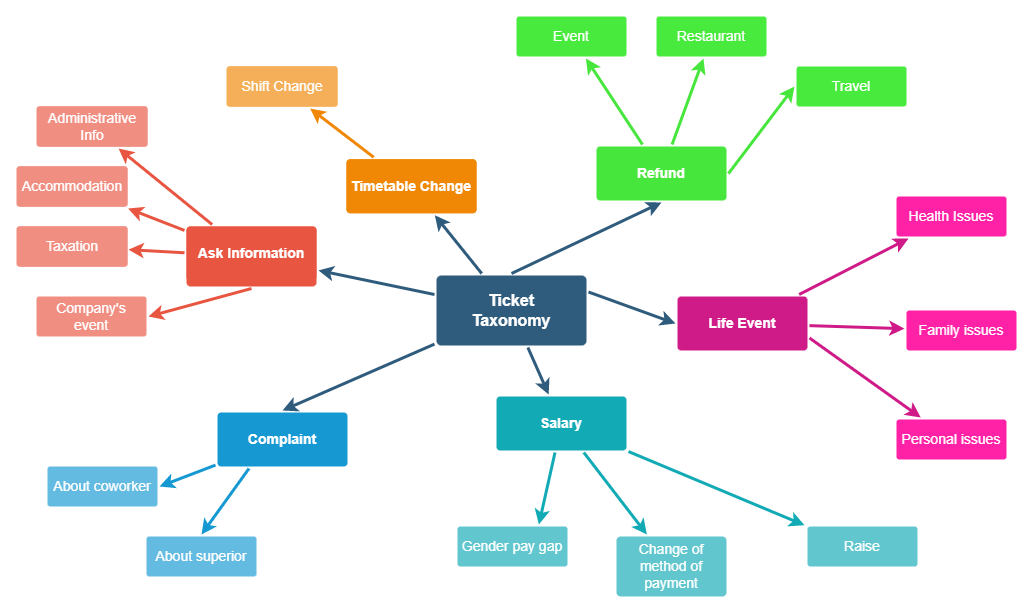
\includegraphics[width=\textwidth]{Taxonomy_Tickets.drawio}

\begin{table}[h]
\resizebox{\textwidth}{!}{
\begin{tabular}{|l|l|l|}
\hline
    Category            & Sub-category   & variables                                   \\ \hline
    Ask Information     & Accomodation   & location, duration                          \\
                        & Taxation       & issue                                       \\
    Complaint           & About coworker & complaint                                   \\
                        & About superior & complaint                                   \\
    Timetable change    & Shift change   & reason\_of\_change, old\_date, new\_date    \\
    Salary              & Salary raise   & old\_salary, new\_salary, increase          \\
                        & Gender pay gap & wage\_gap                                   \\
    Life Event          & Health issues  & disease, number\_of\_days\_of\_sick\_leave  \\
                        & Personal issues  & issue, number\_of\_days                   \\
                        & Family issues  & member\_of\_family, issue, number\_of\_days \\
    Refund              & Event          & date, type\_of\_event                       \\
                        & Travel         & from, to, date, vehicle                     \\
                        & Restaurant     & location, date                              \\ \hline
\end{tabular}
}
\caption{Table of all defined categories and sub-categories}\label{table:categoriesTable}
\end{table}
    

\section{Datasets}
In order to generate tickets, we decided to use real data as a starting point to make them as much realistic as possible. Another reason to use real data is that it makes the dataset useful for use cases such as anonymization. \\
The dataset that we used are all public and available online. In some cases where no datasets were available, we created them manually from personal experience. \\
The datasets are:
\begin{itemize}
    \item \textit{Absenteeism at work Data Set}: contains records of work absences, with the reason of the absence (almost always a disease) and the number of hours of absence. It is used to create the requests of days off for health reasons
    \item \textit{National Occupational Employment and Wage Estimates United States}: estimates of wages in the US calculated with data collected from employers in all industry sectors in metropolitan and nonmetropolitan areas in every state and the District of Columbia. It is used to create the requests of salary raise.
    \item \textit{List of events of life}: list of major events in life. It is used to create the requests of time off due to personal reasons. 
    \item \textit{Gender pay gap in the UK}: dataset of employers with 250 or more employees, comparing men and women’s average pay across the organizations. It is used to create the requests of explanation for the wage gap amongst genders.
    \item \textit{OpenFlights database}: datasets of airports and flights all over the world. It is used for the requests of refund of travels.
    \item \textit{Geonames all cities with a population over 1000}: datasets of all cities of the world with a population over 1000 people. It is used for the requests of information about accommodation.
\end{itemize}

\subsection{Datasets preprocessing}
The \textit{Absenteeism at work Data Set} is the only dataset that contains data about people that is not already grouped and averaged. This means that there is a record in the dataset for each employee request, which contains the personal information of the employee, the reason of the absence and the time of absence in hours. For privacy reasons, we used a Bayesian Network. A Bayesian network is a probabilistic graphical model that measures the conditional dependence structure of a set of random variables based on the Bayes theorem. The features that we have used to build the Bayesian network are the \textit{reason for absence}, the \textit{month of absence} and the \textit{time of absence}.
\\
Using the \textit{Absenteeism at work Data Set} we learn conditional probability distributions from data, to which we add a Laplace noise for differential privacy. Then we can sample new data that follow the original distributions, but that are not equal to the original ones. The absence reasons in the dataset are given as ICD(International Classification of Diseases) codes, to make them more human readable, we picked for each ICD code the corresponding more frequent diseases.

In the \textit{National Occupational Employment and Wage Estimates United States} dataset, we sample employees based on the number of people employed in a certain field. Therefore for example since `Retail Sales Workers` consists of the 5.4\% of the total occupations, then the sampled employee will have the 5.4\% of possibility to have as occupation `Retail Sales Worker`.
The current salary of the employee is calculated adding a Gaussian noise to the average salary of the employee's occupation, and then the salary raise requested is picked randomly between 5\%-10\%.

The ranges of wage gap, used in the tickets regarding explanation for the gender wage gap in the company, are sampled randomly from the dataset \textit{Gender pay gap in the UK}, adding a Gaussian noise for privacy reasons.

To sample the cities for the requests of accomodation, we randomly sample from all the cities with more than 100,000 inhabitants from the country of residence of the synthetic employee. To calculate the duration of the accommodation we pick a random number of months between 1 and 12.

To get data for the category type `refund travel`, we sample randomly one flight from all the flights leaving from the country of the synthetic employee. The data are taken from the \textit{OpenFlights database}.

The complaints about coworkers and superiors and the life events that can affect the work life of a person were handcrafted.

\subsubsection{Bayesian Network}
A Bayesian Model is a machine learning algorithm that is built with Bayes Theorem in mind.  It is based on the probability theory and it enables a machine to learn from the data.
\begin{equation}
    p(A|B) = \frac{p(B|A)p(A)}{p(B)}
\end{equation}
Formally, the Bayesian network is a directed graph G = (V,E) with
\begin{itemize}
    \item A feature for each node i appartenente a V
    \item A conditional probability distribution for each edge, so the edge from feature $i$ to $j$ represents $p(x_j| x_i)$
  \end{itemize}
The base version of a Bayesian network works with discrete variables, however there are also implementations that consider also continuous variables [https://www.jair.org/index.php/jair/article/download/11063/26242/] \\
Building a Bayesian network starting from the \textit{Absenteeism at work Data Set} is relatively easy, we calculate the likelihood distribution $p(x\_i|x\_j) \forall x_i, x_j \in D$ for each other feature $x_j$. As a prior we used a dirichlet distribution. 
[https://mbernste.github.io/files/notes/Psuedocounts.pdf]
https://cs.nyu.edu/~roweis/csc412-2004/notes/lec13x.pdf
We then added pseudocounts to the observed counts in the data used to calculate $p(x_j| x_i)$. This technique is used to diminish the overfitting of data. The values we used for pseudocount is $\gamma=1$. \\
Since we learn the conditional probability distribution from our data, the structure of the network or the conditional probabilities may therefore leak some information on an individual in the dataset. In order to provide strong privacy guarantees and minimize
the re-identification risk, we leverage the notion of differential-privacy: we perturb the data adding a noise sampled from a Laplace distribution 
\begin{equation}
    z \sim Laplace(0, \frac{2 \cdot n_{features}}{\gamma \cdot \epsilon})
\end{equation}
where $\epsilon$ is the privacy budget for differential privacy, which controls the anonymization level.

\begin{equation}
    Pr[M(X) \in Z] \leq e^{\epsilon} \cdot Pr[M(X') \in Z]
\end{equation}
Once the private Bayesian network is built, we can sample new values for all the nodes in the graph. These generated values will have the same distribution and preserve the consistency and statistical properties of the original dataset up to the noise addition which acts as a de-identification barrier. 

    
\section{Ticket Generation}
For each HR ticket, we create a fake employee. For all tickets' categories, the employee has some common features: \textit{name}, \textit{first name}, \textit{last name}, \textit{nationality}, \textit{country}, \textit{email}, \textit{company}, \textit{company's email} and \textit{ticket date}.\\
All these information are created exploiting the Python library \textit{Faker}. The nationality and the company's country are selected from the extendible list \{ USA, Germany, Italy, Spain, France \}. All other information are created accordingly to the country picked. So for example if the country of birth of the employee is Italy, then the generated name will be Italian. \\

Then, once the employees are generated, the information specific to the ticket category, created starting from the open datasets as mentioned before, are concatenated to the general information of the employees. \\
For each ticket category there are distinct templates. In each template there is an initial part that contains the general information of the employee, such as name, surname, company\dots, then some prompts correlated to the category of the ticket and then the textual prompt. \\
Here's an example of a template: \\
\begin{adjustwidth}{1cm}{}
From: \$\{email\} \\
To: \$\{company email\} \\
First name: \$\{first name\}\\
Last name: \$\{last name\}\\
Company: \$\{company\}\\
Date: \$\{ticket date\}\\
Ticket category: \$\{category\}\\
Ticket sub-category: \$\{sub category\} \\
Date start absence: \$\{date start absence\} \\
Reason absence: \$\{reason\} \\ 
\\
Dear Sir/Madame, my name is \$\{name\} and I work at \$\{company\}. I am requesting \textless \textit{generate}\textgreater. I hope \textless \textit{generate}\textgreater. \\ \\
\end{adjustwidth} 
The variables are replaced with the features of the employee, whereas the \textless \textit{generate}\textgreater \space are replaced with text generated by a generative model. The part generated by a pre-trained model are used in a recursive way. This means that the first \textless generate\textgreater \space is replaced with text generated automatically using as prompt everything that precedes it. Then the second \textless generate\textgreater \space will have as prompt the entire ticket, including the text generated previously. The model is forced to generate some text, if no text in an iteration the generation is repeated until the model gives an output not empty.

\subsection{GPT-J}
The generative model used to create the tickets is GPT-J, an open source 6 billion parameter, autoregressive text generation model trained on The Pile dataset released by EleutherAI. \\
The Pile dataset is composed by 22 diverse subsets, which can be grouped in 5 categories:
\begin{itemize}
    \item Academic ( \textit{ArXiv}, \textit{PubMed Central}, ... )
    \item Internet ( \textit{Wikipedia}, \textit{StackExchange}, ... )
    \item Prose ( \textit{Bibliotik}, ... )
    \item Dialogue ( \textit{Subtitles}, ... )
    \item Misc ( \textit{Github}, ... )
\end{itemize}
\vspace{0.5cm}
The parameters used for the generation of the next token are:
\begin{itemize}
    \item \textit{min\_length}: minimum number of words created by a gpt generation
    \item \textit{max\_length}: the max length of the sequence to be generated.  
    \item \textit{top\_k}: the k most likely next words are filtered and the probability mass is redistributed among only these k words.
    
    \item \textit{top\_p}: the next words are sampled from the smallest possible set of words whose cumulative probability exceeds the probability p.
    \item \textit{temperature}: the value $T$ used to module the logits distribution. The higher the value of $T$ the higher the entropy of the logits distribution will be
    \begin{equation}
        p_i = \frac{exp(x_i/T)}{\sum_j exp(x_j/T)}   
    \end{equation}
    \item \textit{repetition\_penalty}: the parameter $\theta$ for repetition penalty. 1.0 means no penalty \\
    Given a list of generated tokens $G$, 
     \begin{equation}
        p_i = \frac{exp(x_i/T \cdot I(i \in G))}{\sum_j exp(x_j/T \cdot I(j \in G))}
    \end{equation}
    \begin{center}
    $I(c) = \theta$ if $c$ is True else 1
    \end{center}

    So the logits distribution of the token change based on if the token has already been generated before.

    \item \textit{length\_penalty}: \textit{length\_penalty} $>$ 0 promotes longer sequences, while \linebreak 
    \textit{length\_penalty} $<$ 0 encourages shorter sequences.
    \item \textit{no\_repeat\_ngram\_size}: If set to int $>$ 0, all ngrams of that size can only occur once \\
    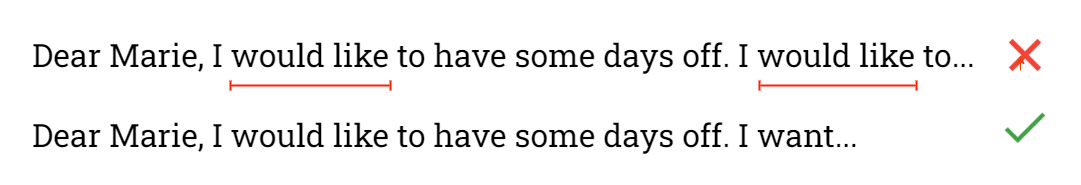
\includegraphics[width=\textwidth]{no_ngram_thesis.drawio.png}
    \item \textit{num\_beams}: Number of beams for beam search. They beams are the number of 'paths' that are considered when choosing the next token \\
    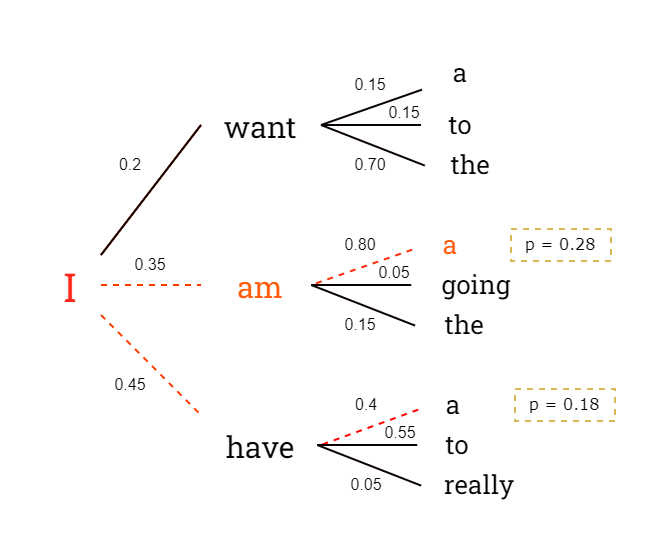
\includegraphics[width=0.5\textwidth]{num_beams.drawio.png}
    \item \textit{do\_sample}: If set to `False` greedy decoding is used ( the most probable token is always chosen). Otherwise, sampling is used ( the next token is chosen sampling from the distribution of possible next tokens )
    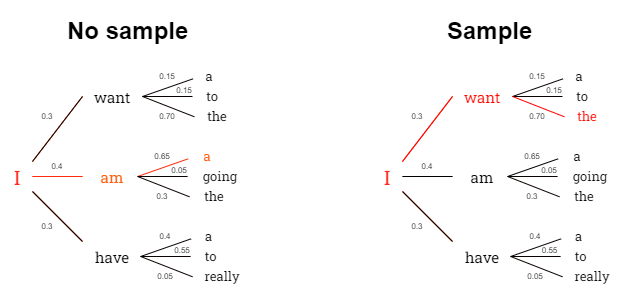
\includegraphics[width=\textwidth]{do_sample.drawio.png}
    \item \textit{bad\_words}: List of words that are not allowed to be generated.
    \item \textit{force\_words}: List of words that must be generated in a generation.
    
\end{itemize}
The default values assigned to the parameters used are shown in \autoref{table:parametersGPTJTable}
\begin{table}[h] 
\centering
\begin{tabular}{|l|l|}
\hline
Parameter          & Value \\ \hline
min length         & 0    \\ 
max length         & 50    \\ 
top k              & 50    \\
top p              & 0.85  \\
repetition penalty & 1.2   \\
temperature        & 1     \\
length penalty     & 1     \\
no repeat ngram size     & 0     \\
num beams &  1 \\
do sample & True \\
bad words & [\space] \\
force words & [\space] \\ \hline
\end{tabular}
\caption{Parameters of GPT-J model}\label{table:parametersGPTJTable}
\end{table}

The GPT architecture is based on the original Transformers paper, which introduced two types of transformers blocks: the encoder block and the decoder block. GPT is assembled by a stack of decoder blocks, which are composed by:
\begin{itemize}
    \item Normalization Layers: a normalization layer \cite{ba2016layer}  normalize all inputs of a neural network across their features. It has been shown that Layer normalization enables smoother gradients, faster training, and better
    generalization accuracy \cite{xu2019understanding}

    $x$: data sample \\
    $d$: dimension of data sample \\
    $y$: output of LayerNorm \\
    $\epsilon$: small number added for stability

    \begin{equation}
        u = \frac{1}{d}\sum_{i=1}^{d}x_i 
    \end{equation}
    \begin{equation}
        \sigma^2 = \frac{1}{d}\sum_{i=1}^{d}(x_ - ui)^2
    \end{equation}
    \begin{equation}
        \hat{x_i} = \frac{x_i - u}{\sqrt{\sigma^2 + \epsilon}}
    \end{equation}
    \begin{equation}
        y = \gamma\hat{x_i} + \beta
    \end{equation}

    where $\gamma$ and $\beta$ are parameters that the model learns.
    \item Masked Self-Attention Layer: attention is a mechanism that allows neural networks to assign a different amount of weight to each token in a sequence and process each token as a weighted average of all other tokens. \\
    In practice three matrixes are calculated:
    \begin{itemize}
        \item $Q$ (Query): the representation of the current token
        \item $K$ (Key): the representation of all the other tokens, which are matched with the current token
        \item $V$ (Value): the representation of all the words, used for the weighted-average
    \end{itemize}
    The $Q$, $K$ and $V$ matrixes are initialized as:
    \begin{itemize}
        \item $Q$ = $W_qX + b_q$ 
        \item $K$ = $W_kX + b_k$ 
        \item $V$ = $W_vX + b_v$
    \end{itemize}
    where $X$ is the input matrix and the other matrixes are randomly initialized and learned by the model.
    Finally, the attention score is calculated with
    \begin{equation}
        Attention(Q,K,V) = softmax(\frac{QK^T}{\sqrt{d}})V
    \end{equation}
    where $d$ is a normalization factor equivalent to the embeddings dimension \\
    The masked self-attention is a modified version of self-attention where all the tokens that appear after the current one are set to $0$, in order not to let the model know any information regarding the tokens at the next positions. This is fundemantel when training generative models such as GPT, whose scope is to predict the successive tokens.
    \item Feed Forward Neural Network Layer: Used to add non-linearity to the transformer block
\end{itemize}
Compared to GPT-3, GPT-J has two minor architectural differences\cite[]{gpt-j}:
\begin{itemize}
    \item Rotary Embedding
    \item The attention layer and the feedforward layer in parallel for decreased communication
\end{itemize}

\subsection{Rotary Embedding}
Rotary 

\begin{figure}[h] 
    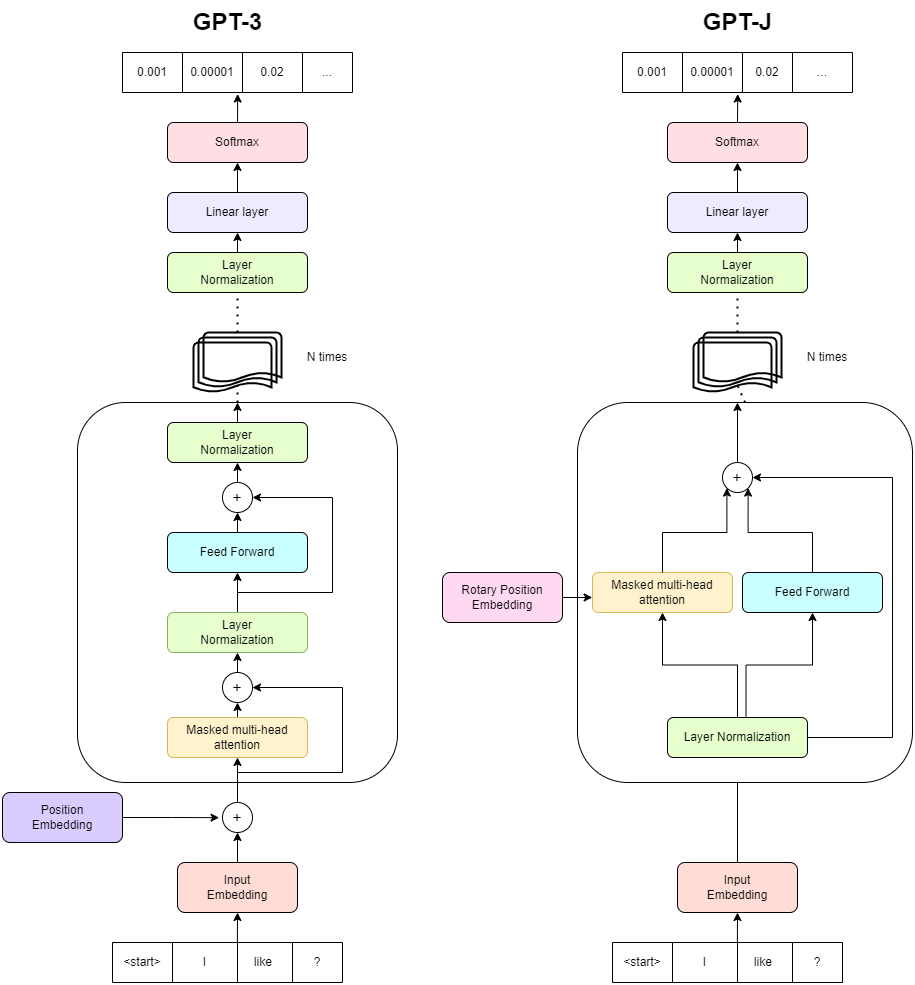
\includegraphics[width=\textwidth]{gptJ_vs_gpt_architecture.drawio.png}
    \caption{GPT-3 and GPT-J architectures compared}
    \label{GPT-architectures}
\end{figure}    



\section{Dataset analysis}


\section{Experiments}


\bibliography{biblio} 
\bibliographystyle{ieeetr}
    

\end{document}